\documentclass[11pt,letterpaper]{article}

% --- PAQUETES BÁSICOS Y CODIFICACIÓN ---
\usepackage[utf8]{inputenc}
\usepackage[T1]{fontenc}
\usepackage[spanish,es-tabla]{babel}
\usepackage{lmodern}
\usepackage{microtype}

% --- MÁRGENES Y DISEÑO DE PÁGINA ---
\usepackage[letterpaper, top=2.5cm, bottom=2.5cm, left=2.5cm, right=2.5cm]{geometry}
\usepackage{fancyhdr}
\usepackage{titlesec}
\usepackage{setspace}
\setstretch{1.15}

% --- GRÁFICOS Y RUTA DE IMÁGENES ---
\usepackage{graphicx}
% Configuración para Overleaf: Busca en la carpeta imagenes/ o en el directorio raíz
\graphicspath{{imagenes/}{./}}

% --- TABLAS Y FORMATO ---
\usepackage{booktabs}
\usepackage{tabularx}
\usepackage{array}
\usepackage{multirow}
\usepackage{colortbl}

% --- COLORES Y CAJAS DESTACADAS ---
\usepackage{xcolor}
\definecolor{utbblue}{RGB}{37, 99, 235}
\definecolor{darkblue}{RGB}{30, 58, 138}
\definecolor{headerblue}{RGB}{224, 242, 254}
\definecolor{borderblue}{RGB}{147, 197, 253}
\definecolor{darkslate}{RGB}{15, 23, 42}
\definecolor{lightgray}{RGB}{248, 250, 252}
\definecolor{bordergray}{RGB}{203, 213, 225}
\definecolor{succgreen}{RGB}{22, 101, 52}
\definecolor{alertred}{RGB}{153, 27, 27}
\definecolor{codebg}{RGB}{15, 23, 42}
\definecolor{codefg}{RGB}{248, 250, 252}

\usepackage[most]{tcolorbox}
\newtcolorbox{legalcallout}{
    colback=yellow!5!white,
    colframe=orange!75!black,
    fonttitle=\bfseries,
    title=Cláusula de Deslinde Legal (Ley 1480 de 2011),
    arc=2mm,
    boxrule=1pt,
    left=3mm, right=3mm, top=2mm, bottom=2mm
}

\newtcolorbox{successcallout}{
    colback=green!5!white,
    colframe=green!60!black,
    fonttitle=\bfseries,
    title=Declaración de Aprobación y Alcance FDD,
    arc=2mm,
    boxrule=1pt,
    left=3mm, right=3mm, top=2mm, bottom=2mm
}

\newtcolorbox{diffbeforebox}{
    colback=red!4!white,
    colframe=red!60!black,
    fonttitle=\bfseries\small,
    title=Código Antes (Vulnerable),
    arc=1mm,
    boxrule=0.8pt,
    left=2mm, right=2mm, top=2mm, bottom=2mm
}

\newtcolorbox{diffafterbox}{
    colback=green!4!white,
    colframe=green!60!black,
    fonttitle=\bfseries\small,
    title=Código Corregido (Con Guarda),
    arc=1mm,
    boxrule=0.8pt,
    left=2mm, right=2mm, top=2mm, bottom=2mm
}

% --- CÓDIGO FUENTE (LISTINGS) ---
\usepackage{listings}
\lstdefinestyle{mystyle}{
    backgroundcolor=\color{codebg},
    basicstyle=\ttfamily\footnotesize\color{codefg},
    breakatwhitespace=false,
    breaklines=true,
    captionpos=b,
    keepspaces=true,
    numbers=none,
    showspaces=false,
    showstringspaces=false,
    showtabs=false,
    tabsize=2,
    frame=single,
    rulecolor=\color{bordergray}
}
\lstset{style=mystyle}

% --- NOTAS DE FIGURA APA 7 ---
\usepackage{caption}
\captionsetup[figure]{labelfont={bf}, textfont={it}, labelsep=period, singlelinecheck=false}
\captionsetup[table]{labelfont={bf}, textfont={it}, labelsep=period, singlelinecheck=false}
\newcommand{\figurenote}[1]{\vspace{2mm}\small\noindent\textit{Nota.} #1\vspace{4mm}}

% --- ENLACES HIPERTEXTO ---
\usepackage{hyperref}
\hypersetup{
    colorlinks=true,
    linkcolor=utbblue,
    citecolor=darkblue,
    urlcolor=utbblue,
    pdfauthor={Alejandro David Paternina Bermejo y Johan Sebastian Brieva Fernandez},
    pdftitle={Proyecto de Aula Motrik - MVP Final}
}

% --- ENCABEZADOS Y PIES ---
\pagestyle{fancy}
\fancyhf{}
\fancyhead[L]{\small\textsf{Ingeniería de Software · Proyecto de Aula Motrik (MVP)}}
\fancyhead[R]{\small\textsf{UTB — 2026}}
\fancyfoot[C]{\thepage}
\renewcommand{\headrulewidth}{0.4pt}
\renewcommand{\footrulewidth}{0.4pt}

% Formato de secciones
\titleformat{\section}{\Large\bfseries\color{darkslate}}{\thesection.}{0.8em}{}[\titlerule]
\titleformat{\subsection}{\large\bfseries\color{darkblue}}{\thesubsection.}{0.6em}{}
\titleformat{\subsubsection}{\normalsize\bfseries\color{darkslate}}{\thesubsubsection.}{0.5em}{}

% Sangría francesa para APA 7
\newenvironment{hangparas}[2]{\setlength{\parindent}{\z@}\everypar{\parindent#1\hangindent#2}}{\par}

\begin{document}

% ==========================================
% PORTADA INSTITUCIONAL
% ==========================================
\begin{titlepage}
    \centering
    \vspace*{0.5cm}
    
    % Logo UTB
    
\includegraphics[height=2.2cm]{logo_utb.png}\\[0.6cm]
    
    {\scshape\Large Universidad Tecnológica de Bolívar\par}
    \vspace{0.2cm}
    {\scshape\large Facultad de Ingeniería\par}
    \vspace{0.1cm}
    {\large Programa de Ingeniería de Software · Grupo 1208\par}
    \vspace{1.5cm}
    
    \noindent\rule{\linewidth}{1.5pt}\\[0.4cm]
    {\large\bfseries\color{utbblue} PROYECTO DE AULA — TERCER CORTE (MVP FINAL)\par}\vspace{0.3cm}
    {\huge\bfseries Motrick\par}\vspace{0.4cm}
    {\large Plataforma Centralizada para la Gestión de Mantenimiento Vehicular, Directorio de Talleres Especializados y Catálogo de Repuestos\par}
    \noindent\rule{\linewidth}{1.5pt}
    
    \vspace{1.8cm}
    
    \begin{minipage}[t]{0.48\textwidth}
        \textbf{Estudiantes Desarrolladores:}\\[0.2cm]
        Alejandro David Paternina Bermejo\\
        \textit{Código: T00078032}\\[0.3cm]
        Johan Sebastian Brieva Fernandez\\
        \textit{Código: T00077809}
    \end{minipage}
    \hfill
    \begin{minipage}[t]{0.48\textwidth}
        \raggedleft
        \textbf{Docente Evaluador:}\\[0.2cm]
        Aisner Jose Marrugo Juliao\\
        \textit{Docente Titular de Ingeniería de Software}\\[0.4cm]
        \textbf{Semestre Académico:}\\
        Semestre 8 · Periodo 2026
    \end{minipage}
    
    \vfill
    {\large Cartagena de Indias, Bolívar · Octubre de 2026\par}
\end{titlepage}

% ==========================================
% TABLA DE CONTENIDO
% ==========================================
\thispagestyle{plain}
\tableofcontents
\newpage

% ==========================================
% CAPÍTULO 1
% ==========================================
\section{Propósito del Proyecto de Aula y Marco de Negocio}

El Proyecto de Aula busca integrar los conocimientos y prácticas trabajados en la asignatura de \textbf{Ingeniería de Software} mediante el desarrollo incremental de una solución a un problema real y representativo de la industria automotriz. El proyecto se ejecutó durante el segundo y tercer corte evaluativo, consolidando evidencias completas de análisis, diseño, construcción, pruebas en base de datos real, gestión ágil del trabajo y liberación del Producto Mínimo Viable (MVP).

\subsection{Descripción del Problema}
Encontrar un mecánico de confianza, cotizar el repuesto exacto y llevar un registro organizado de las intervenciones mecánicas suele ser un desafío constante para los conductores en Colombia. La información se encuentra fragmentada, los precios varían sin control y, en muchas ocasiones, el usuario carece de certeza sobre la compatibilidad de un componente o la idoneidad del taller.

\subsection{Solución Propuesta (Alcance del MVP)}
\textbf{Motrick} es una plataforma web full-stack diseñada para centralizar la gestión vehicular. Para garantizar la viabilidad dentro del calendario académico, el alcance del MVP se estructura en tres módulos clave:
\begin{itemize}
    \item \textbf{Directorio de Servicios Especializados:} Catálogo de mecánicos y talleres filtrable por especialidad técnica, con cálculo de calificación promedio y solicitud de verificación formal de talleres.
    \item \textbf{Buscador y Catálogo de Repuestos:} Módulo de consulta categorizado y filtrable por modelo vehicular con validación de compatibilidad técnica.
    \item \textbf{Bitácora de Mantenimiento y Garaje Digital:} Espacio donde el propietario registra los servicios preventivos y correctivos, controlando odómetro, piezas actualizadas, costos y fechas de vencimiento de SOAT y revisión técnico-mecánica.
\end{itemize}

\subsection{Alcance y Restricciones Tecnológicas}
\begin{itemize}
    \item \textbf{Persistencia de Datos:} El sistema opera conectado a una base de datos relacional PostgreSQL alojada en Supabase Cloud, implementando políticas de seguridad a nivel de fila (\textit{Row Level Security} - RLS).
    \item \textbf{Enlace Directo con Talleres sin Intermediación Financiera (RNF-03):} En estricto apego al modelo B2B y al Art. 53 de la Ley 1480 de 2011, Motrik no capta pagos ni intermedia cobros por repuestos o mano de obra. El catálogo conecta al conductor directamente con el taller especializado en Cartagena (vía WhatsApp y llamada directa) para coordinar la compra, retiro o instalación física.
\end{itemize}

\subsection{Arquitectura y Tecnologías}
La arquitectura se fundamenta en un ecosistema unificado basado en JavaScript y TypeScript estricto:
\begin{itemize}
    \item \textbf{Framework Full-Stack:} Next.js 14 con arquitectura App Router, React 18 y Tailwind CSS para diseño responsivo con soporte nativo de modo oscuro/claro.
    \item \textbf{Backend y Persistencia:} Supabase (BaaS) sobre PostgreSQL 15, garantizando integridad referencial, restricciones de dominio CHECK y autenticación.
\end{itemize}

\subsection{Modelo de Negocio y Marco Jurídico Institucional}
Motrick implementa un modelo de monetización B2B sustentado en membresías de visibilidad y verificación para talleres mecánicos, y pauta publicitaria nativa vehicular, \textbf{descartando expresamente el cobro de comisiones sobre reparaciones mecánicas}.

\subsubsection{Prevención de Solidaridad Jurídica y Portal de Contacto (Art. 53, Ley 1480 de 2011)}
De acuerdo con el \textbf{Artículo 53 de la Ley 1480 de 2011 (Estatuto del Consumidor en Colombia)}, la plataforma califica como \textbf{portal de contacto e intermediación informativa}. Si Motrick recaudara el valor del servicio de mano de obra o comisionara sobre el arreglo mecánico, la Superintendencia de Industria y Comercio (SIC) la consideraría prestador solidario, debiendo responder económicamente ante fallas mecánicas, averías colaterales o garantías no atendidas por el taller.

Al limitar los ingresos al canon de visibilidad y verificación documental, la relación contractual por el servicio automotriz se suscribe directa y exclusivamente entre el propietario del vehículo y el taller mecánico contratado.

\begin{legalcallout}
\textit{«Motrick opera bajo la figura de portal de contacto (Art. 53, Ley 1480 de 2011). La plataforma no ejecuta diagnósticos mecánicos, no provee mano de obra ni actúa como garante solidario de los trabajos realizados por los talleres listados. La contratación de servicios automotrices, su calidad y cumplimiento de garantías recaen exclusivamente en el establecimiento seleccionado por el usuario.»}
\end{legalcallout}

\subsubsection{Publicidad Nativa Contextual y Política de Brand Safety (RNF-04)}
Como línea secundaria de sostenimiento, se habilitan espacios pasivos en los márgenes y zonas blancas de la interfaz, alineados con los \textbf{Artículos 29 y 30 de la Ley 1480 de 2011 (protección contra publicidad engañosa)}:
\begin{itemize}
    \item \textbf{Relevancia temático-vehicular:} Solo se admiten anunciantes de servicios afines (SOAT digital, revisión técnico-mecánica en Centros CDA aliados, escáneres OBD2 Bluetooth y telepeaje).
    \item \textbf{Cero intrusión (UX):} Se vetan pop-ups, modales bloqueantes o banners con sonido, garantizando cero desplazamiento visual (\textit{Cumulative Layout Shift} = 0).
    \item \textbf{Seguridad de marca (Brand Safety):} Quedan prohibidos juegos móviles, apuestas deportivas, esquemas de inversión y contenido adulto (+18). Toda inserción cuenta con el distintivo gráfico visible y obligatorio \textbf{"Patrocinado"}.
\end{itemize}

\newpage

% ==========================================
% CAPÍTULO 2
% ==========================================
\section{Identificación de Interesados (Stakeholders)}

Para garantizar una adecuada gestión de expectativas y cobertura de requisitos, se identificaron cuatro actores clave del ecosistema de Motrick:

\begin{table}[h!]
\centering
\small
\begin{tabularx}{\textwidth}{p{3.2cm}Xp{6.5cm}}
\toprule
\textbf{Nombre / Rol} & \textbf{Relación con el Proyecto} & \textbf{Principales Necesidades / Expectativas} \\
\midrule
\textbf{Usuario Final}\newline (Propietario de vehículo) & Actor principal. Interactúa con la interfaz para buscar servicios, repuestos y registrar la bitácora técnica de sus vehículos. & • Encontrar mecánicos verificados y confiables.\newline • Cotizar repuestos con compatibilidad técnica garantizada.\newline • Llevar un historial digital permanente de mantenimientos. \\
\addlinespace
\textbf{Mecánico o Taller}\newline (Proveedor de servicio) & Interesado clave. Su información nutre el directorio de servicios, solicita verificación y recibe clientes calificados. & • Mayor visibilidad digital para captar clientes en Cartagena.\newline • Destacar su especialidad técnica (Frenos, Motor, etc.).\newline • Construir reputación comercial verificada mediante reseñas. \\
\addlinespace
\textbf{Administrador}\newline (Equipo Motrick) & Gestiona la plataforma, audita la documentación fiscal de talleres (NIT/RUT) y supervisa el catálogo de repuestos. & • Controlar el catálogo de repuestos automotrices.\newline • Auditar y otorgar la insignia de "Taller Verificado".\newline • Moderar valoraciones y asegurar el cumplimiento normativo. \\
\addlinespace
\textbf{Docente / Evaluador}\newline (Stakeholder académico) & Guía, audita y califica el desarrollo del proyecto de aula en la Universidad Tecnológica de Bolívar. & • Evidenciar la aplicación de técnicas de elicitación.\newline • Validar pruebas reales ejecutadas contra base de datos.\newline • Evaluar la disciplina en gestión ágil (FDD y control Git). \\
\bottomrule
\end{tabularx}
\caption{Matriz de Caracterización de Interesados (Stakeholders) de Motrick.}
\end{table}

% ==========================================
% CAPÍTULO 3
% ==========================================
\section{Técnicas de Elicitación Aplicadas}

Para fundamentar técnicamente los módulos del sistema, se aplicaron tres metodologías formales de levantamiento de requisitos:

\subsection{Benchmarking (Análisis de Soluciones Similares)}
Se analizaron aplicaciones líderes en gestión y servicios automotrices (Drivvo, Autolab y MercadoLibre Repuestos). Conclusión: las aplicaciones existentes resuelven problemas de forma fragmentada. La ventaja competitiva de Motrick radica en \textbf{centralizar en una sola plataforma} el directorio confiable, el catálogo compatible y la bitácora técnica.

\subsection{Encuesta a Usuarios Potenciales (49 Conductores)}
Se diseñó y aplicó un cuestionario digital a 49 conductores activos en Cartagena, indagando sobre hábitos de compra de repuestos, selección de talleres y control del historial de reparaciones.

\subsection{Revisión Documental y Normativa del Sector Automotor}
Se articularon estudios gremiales de ASOPARTES, informes internacionales de la American Automobile Association (AAA, 2016) sobre la desconfianza del consumidor en la reparación vehicular, y el marco legal del Estatuto del Consumidor (Ley 1480 de 2011).

\newpage

% ==========================================
% CAPÍTULO 4
% ==========================================
\section{Muestras de las Herramientas Utilizadas y Evidencias del Sector}

\subsection{Cuadro Comparativo de Benchmarking}

\begin{table}[h!]
\centering
\small
\begin{tabularx}{\textwidth}{p{2.5cm}XXp{4.2cm}}
\toprule
\textbf{Plataforma} & \textbf{Puntos Fuertes} & \textbf{Limitaciones Detectadas} & \textbf{Diferencial Estratégico de Motrick} \\
\midrule
\textbf{Drivvo} & Excelente registro de kilometraje y consumo de combustible. & No cuenta con directorio de talleres ni catálogo de piezas. & Motrick unifica bitácora con directorio especializado y catálogo. \\
\addlinespace
\textbf{Autolab} & Red propia de talleres y estandarización de servicios mecánicos. & Modelo cerrado limitado a su propia franquicia de talleres. & Motrick es un ecosistema abierto con validación y reseñas auditadas. \\
\addlinespace
\textbf{MercadoLibre} & Catálogo masivo de autopartes y despacho a domicilio. & Alta tasa de error en compatibilidad y nula gestión de bitácora. & Motrick categoriza repuestos según modelo vehicular y bitácora. \\
\bottomrule
\end{tabularx}
\caption{Matriz Comparativa de Benchmarking Competitivo.}
\end{table}

\subsection{Resultados Consolidados de la Encuesta a 49 Usuarios}
El instrumento digital evidenció datos contundentes sobre los hábitos de los conductores:
\begin{itemize}
    \item \textbf{Búsqueda de Mecánicos:} El \textbf{91.8\%} depende exclusivamente de la recomendación informal ("boca a boca"), demostrando la ausencia de herramientas digitales confiables.
    \item \textbf{Filtros por Especialidad y Reseñas:} El \textbf{98.0\%} consideró "Muy útil" o "Útil" consultar valoraciones y filtrar mecánicos por especialidad antes de acudir.
    \item \textbf{Dificultad en Repuestos:} El \textbf{53.1\%} manifestó que su mayor temor al comprar autopartes es \textit{"Tener certeza de la compatibilidad con mi vehículo"}.
    \item \textbf{Control de Historial:} El \textbf{75.5\%} no lleva ningún registro o guarda facturas sueltas en la guantera con riesgo de pérdida.
    \item \textbf{Aceptación de la Propuesta:} El \textbf{100\%} de los encuestados afirmó que usaría una plataforma que centralice talleres, repuestos compatibles y bitácora digital.
\end{itemize}

\subsection{Hallazgos de la Revisión Documental del Sector}
\begin{itemize}
    \item \textbf{Desconfianza Estructural (Estudio AAA):} Dos tercios de los conductores desconfían de los talleres por temor a cobros inflados. Motrick mitiga esto mediante el sistema de valoraciones auditadas y el canal de verificación documental (RF-05).
    \item \textbf{Incompatibilidad de Autopartes (ASOPARTES):} La compra desinformada de repuestos paraliza los talleres. Motrick soluciona esto categorizando piezas compatibles con el modelo exacto (RF-04).
    \item \textbf{Asimetría Informativa:} La ausencia de bitácora provoca diagnósticos redundantes y costosos. Motrick transfiere el control digital del historial al usuario (RF-01).
\end{itemize}

\newpage

% ==========================================
% CAPÍTULO 5
% ==========================================
\section{Especificación de Requerimientos de Software}

Con base en la elicitación, se formalizaron cinco requerimientos funcionales (RF) y cuatro requerimientos no funcionales (RNF) para el MVP:

\subsection{Requerimientos Funcionales (RF)}

% RF-01
\begin{table}[h!]
\centering
\small
\begin{tabularx}{\textwidth}{p{3.5cm}X}
\toprule
\multicolumn{2}{l}{\textbf{\color{darkblue}Ficha Técnica: RF-01 — Registro y Control de Mantenimiento en Bitácora}} \\
\midrule
\textbf{Identificador} & \textbf{RF-01} \\
\textbf{Nombre} & Registrar y gestionar mantenimiento en bitácora vehicular \\
\textbf{Descripción} & El sistema debe permitir al usuario propietario registrar mantenimientos especificando vehículo, fecha, odómetro, título del servicio, notas, taller ejecutor y repuesto opcional. \\
\textbf{Fuente} & Encuesta a Usuarios (Pregunta 4: 75.5\% sin registro organizado) y Revisión Documental. \\
\textbf{Prioridad} & Alta \\
\textbf{Criterio de Aceptación} & El registro se almacena en la tabla \texttt{registros\_bitacora} de Supabase. Si el odómetro ingresado es menor al actual, la interfaz bloquea el registro (Defecto D1 corregido). \\
\bottomrule
\end{tabularx}
\end{table}

% RF-02
\begin{table}[h!]
\centering
\small
\begin{tabularx}{\textwidth}{p{3.5cm}X}
\toprule
\multicolumn{2}{l}{\textbf{\color{darkblue}Ficha Técnica: RF-02 — Directorio de Talleres con Filtros de Especialidad}} \\
\midrule
\textbf{Identificador} & \textbf{RF-02} \\
\textbf{Nombre} & Filtrar directorio de talleres por especialidad técnica \\
\textbf{Descripción} & El sistema debe listar mecánicos y talleres permitiendo aplicar filtros por especialidad (Frenos, Motor, Suspensión, Transmisión, Eléctrico) y zona geográfica en Cartagena. \\
\textbf{Fuente} & Encuesta a Usuarios (Pregunta 2: 98\% de interés) y Benchmarking. \\
\textbf{Prioridad} & Alta \\
\textbf{Criterio de Aceptación} & La consulta a \texttt{mecanicos} filtra dinámicamente mediante \texttt{ILIKE} sobre la especialidad y actualiza la cuadrícula de talleres en tiempo real. \\
\bottomrule
\end{tabularx}
\end{table}

% RF-03
\begin{table}[h!]
\centering
\small
\begin{tabularx}{\textwidth}{p{3.5cm}X}
\toprule
\multicolumn{2}{l}{\textbf{\color{darkblue}Ficha Técnica: RF-03 — Consulta de Valoraciones y Reseñas de Mecánicos}} \\
\midrule
\textbf{Identificador} & \textbf{RF-03} \\
\textbf{Nombre} & Consultar valoraciones y reseñas de mecánicos \\
\textbf{Descripción} & El perfil de cada taller debe desplegar una calificación promedio (1.0 a 5.0 estrellas) calculada a partir de las reseñas emitidas por clientes verificados. \\
\textbf{Fuente} & Revisión Documental (Mitigación de desconfianza según estudio AAA). \\
\textbf{Prioridad} & Media / Alta \\
\textbf{Criterio de Aceptación} & El sistema renderiza el promedio de estrellas y lista las reseñas. La tabla \texttt{valoraciones} en PostgreSQL protege el rango estricto mediante restricción CHECK. \\
\bottomrule
\end{tabularx}
\end{table}

\newpage

% RF-04
\begin{table}[h!]
\centering
\small
\begin{tabularx}{\textwidth}{p{3.5cm}X}
\toprule
\multicolumn{2}{l}{\textbf{\color{darkblue}Ficha Técnica: RF-04 — Catálogo de Repuestos con Compatibilidad Vehicular}} \\
\midrule
\textbf{Identificador} & \textbf{RF-04} \\
\textbf{Nombre} & Buscar repuestos compatibles según el modelo vehicular \\
\textbf{Descripción} & El sistema debe consultar un catálogo de piezas automotrices categorizadas, indicando mediante un badge gráfico si el repuesto es compatible con el vehículo activo del usuario. \\
\textbf{Fuente} & Encuesta a Usuarios (Pregunta 3: 53.1\% teme incompatibilidad) e informes de ASOPARTES. \\
\textbf{Prioridad} & Alta \\
\textbf{Criterio de Aceptación} & El catálogo consulta la tabla \texttt{repuestos} en Supabase y compara la columna \texttt{compatibilidad} con la marca y modelo del automóvil activo. \\
\bottomrule
\end{tabularx}
\end{table}

% RF-05
\begin{table}[h!]
\centering
\small
\begin{tabularx}{\textwidth}{p{3.5cm}X}
\toprule
\multicolumn{2}{l}{\textbf{\color{darkblue}Ficha Técnica: RF-05 — Verificación y Validación Documental de Talleres}} \\
\midrule
\textbf{Identificador} & \textbf{RF-05} \\
\textbf{Nombre} & Verificación y validación de talleres mecánicos \\
\textbf{Descripción} & El sistema debe disponer de un canal para que los talleres soliciten una insignia de acreditación suministrando NIT/RUT, razón social, dirección física y teléfono de contacto. El Administrador valida la autenticidad de los datos para otorgar la insignia de taller verificado, y el directorio permite filtrar según este criterio. \\
\textbf{Fuente} & Elicitación: Mitigación de desconfianza del usuario (Estudio AAA) y modelo de membresías B2B. \\
\textbf{Prioridad} & Media \\
\textbf{Criterio de Aceptación} & El perfil del taller en \texttt{/directorio} muestra la insignia gráfica tras su confirmación en base de datos, y el filtro "Solo verificados" actualiza el listado en tiempo real. \\
\bottomrule
\end{tabularx}
\end{table}

\subsection{Requerimientos No Funcionales (RNF)}

% RNF-01
\begin{table}[h!]
\centering
\small
\begin{tabularx}{\textwidth}{p{3.5cm}X}
\toprule
\multicolumn{2}{l}{\textbf{\color{darkblue}Ficha Técnica: RNF-01 — Arquitectura Full-Stack en Next.js y Modern UX}} \\
\midrule
\textbf{Identificador} & \textbf{RNF-01} \\
\textbf{Nombre} & Arquitectura Full-Stack en Next.js y Modern UX \\
\textbf{Descripción} & La plataforma debe construirse sobre Next.js 14 con App Router, React 18, TypeScript estricto y Tailwind CSS, soportando tema claro/oscuro y componentes accesibles Radix UI. \\
\textbf{Fuente} & Estándar arquitectónico de Motrick. \\
\textbf{Prioridad} & Alta \\
\textbf{Criterio de Aceptación} & Compilación de producción (\texttt{npm run build}) exitosa con 0 errores de TypeScript y pre-renderizado estático de rutas. \\
\bottomrule
\end{tabularx}
\end{table}

% RNF-02
\begin{table}[h!]
\centering
\small
\begin{tabularx}{\textwidth}{p{3.5cm}X}
\toprule
\multicolumn{2}{l}{\textbf{\color{darkblue}Ficha Técnica: RNF-02 — Persistencia en Supabase (PostgreSQL) con RLS}} \\
\midrule
\textbf{Identificador} & \textbf{RNF-02} \\
\textbf{Nombre} & Persistencia y Base de Datos en Supabase (PostgreSQL) con RLS \\
\textbf{Descripción} & El sistema debe persistir datos relacionales en PostgreSQL alojado en Supabase, implementando políticas Row-Level Security (RLS) para proteger datos de bitácora y vehículos. \\
\textbf{Fuente} & Requerimientos de seguridad y persistencia cloud. \\
\textbf{Prioridad} & Alta \\
\textbf{Criterio de Aceptación} & Tablas relacionales protegidas con RLS; consultas anónimas limitadas a lectura de catálogo público y directorios autorizados. \\
\bottomrule
\end{tabularx}
\end{table}

\newpage

% RNF-03
\begin{table}[h!]
\centering
\small
\begin{tabularx}{\textwidth}{p{3.5cm}X}
\toprule
\multicolumn{2}{l}{\textbf{\color{darkblue}Ficha Técnica: RNF-03 — Enlace Directo con Talleres sin Intermediación Financiera}} \\
\midrule
\textbf{Identificador} & \textbf{RNF-03} \\
\textbf{Nombre} & Enlace directo con taller aliado para repuestos (Sin intermediación financiera) \\
\textbf{Descripción} & La plataforma no intermedia cobros ni procesa pagos bancarios por repuestos. El sistema provee un canal de enlace directo con el taller autorizado en Cartagena (vía WhatsApp y enlace telefónico), transfiriendo las especificaciones de compatibilidad vehicular para coordinar la disponibilidad, compra y montaje presencial. \\
\textbf{Fuente} & Modelo de Negocio B2B y Blindaje Jurídico (Art. 53, Ley 1480 de 2011). \\
\textbf{Prioridad} & Media \\
\textbf{Criterio de Aceptación} & El modal de contacto asigna automáticamente el taller idóneo en Cartagena según la especialidad de la pieza, genera el mensaje técnico estructurado sin solicitar datos financieros y provee acceso al perfil del taller en el directorio (Defecto D2 corregido). \\
\bottomrule
\end{tabularx}
\end{table}

\vspace{0.4cm}

% RNF-04
\begin{table}[h!]
\centering
\small
\begin{tabularx}{\textwidth}{p{3.5cm}X}
\toprule
\multicolumn{2}{l}{\textbf{\color{darkblue}Ficha Técnica: RNF-04 — Publicidad Nativa Contextual y Brand Safety}} \\
\midrule
\textbf{Identificador} & \textbf{RNF-04} \\
\textbf{Nombre} & Visualización de publicidad nativa contextual no invasiva \\
\textbf{Descripción} & La interfaz debe desplegar inserciones publicitarias pasivas integradas orgánicamente en el diseño (componente \texttt{SponsoredCard}) para servicios vehiculares aliados, con la etiqueta visible "Patrocinado", política de Brand Safety y sin ventanas emergentes. \\
\textbf{Fuente} & Modelo de negocio de la plataforma, Art. 29 y 30 de la Ley 1480 de 2011, y atributos de usabilidad (UX). \\
\textbf{Prioridad} & Baja / Media \\
\textbf{Criterio de Aceptación} & Las tarjetas respetan los tokens cromáticos de Tailwind CSS en temas claro y oscuro, garantizan desplazamiento visual cero ($CLS = 0$) y no interfieren en los formularios ni generan redirecciones automáticas. \\
\bottomrule
\end{tabularx}
\end{table}

% ==========================================
% CAPÍTULO 6
% ==========================================
\section{Priorización de Requerimientos y Alcance Funcional (FDD)}

Aplicando los principios de la metodología \textbf{Feature-Driven Development (FDD)}, los requerimientos se clasificaron en tres niveles de entrega:
\begin{itemize}
    \item \textbf{Prioridad Alta (Obligatorios para el MVP):} RF-01 (Bitácora), RF-02 (Directorio), RF-04 (Repuestos compatibles), RNF-01 (Next.js) y RNF-02 (Supabase).
    \item \textbf{Prioridad Media (Valor agregado indispensable):} RF-03 (Valoraciones), RF-05 (Verificación de talleres), RNF-03 (Enlace directo con talleres) y RNF-04 (Pauta nativa contextual).
    \item \textbf{Prioridad Baja (Alcance futuro post-MVP):} Integración en tiempo real con inventarios de repuestos de talleres y sistemas POS presenciales aliados.
\end{itemize}

\begin{successcallout}
\textbf{Cumplimiento de Alcance:} Al cierre de la iteración final, el \textbf{100\% de los requerimientos de Prioridad Alta y Media} se encuentran completamente desarrollados, integrados y probados.
\end{successcallout}

\newpage

% ==========================================
% CAPÍTULO 7
% ==========================================
\section{Modelado UML y Matriz de Validación Metodológica}

\subsection{Diagrama de Casos de Uso Actualizado (Figura 1)}
El diagrama de casos de uso fue actualizado formalmente para incorporar el actor \textbf{Mecánico / Taller} (con el caso de uso \textit{Solicitar verificación de taller}) y el actor \textbf{Administrador} (con la moderación de directorio, catálogo y aprobación de insignias fiscales), así como las relaciones \texttt{<<extend>>} hacia el contacto directo por WhatsApp y la vinculación de piezas en bitácora:

\begin{figure}[h!]
    \centering
    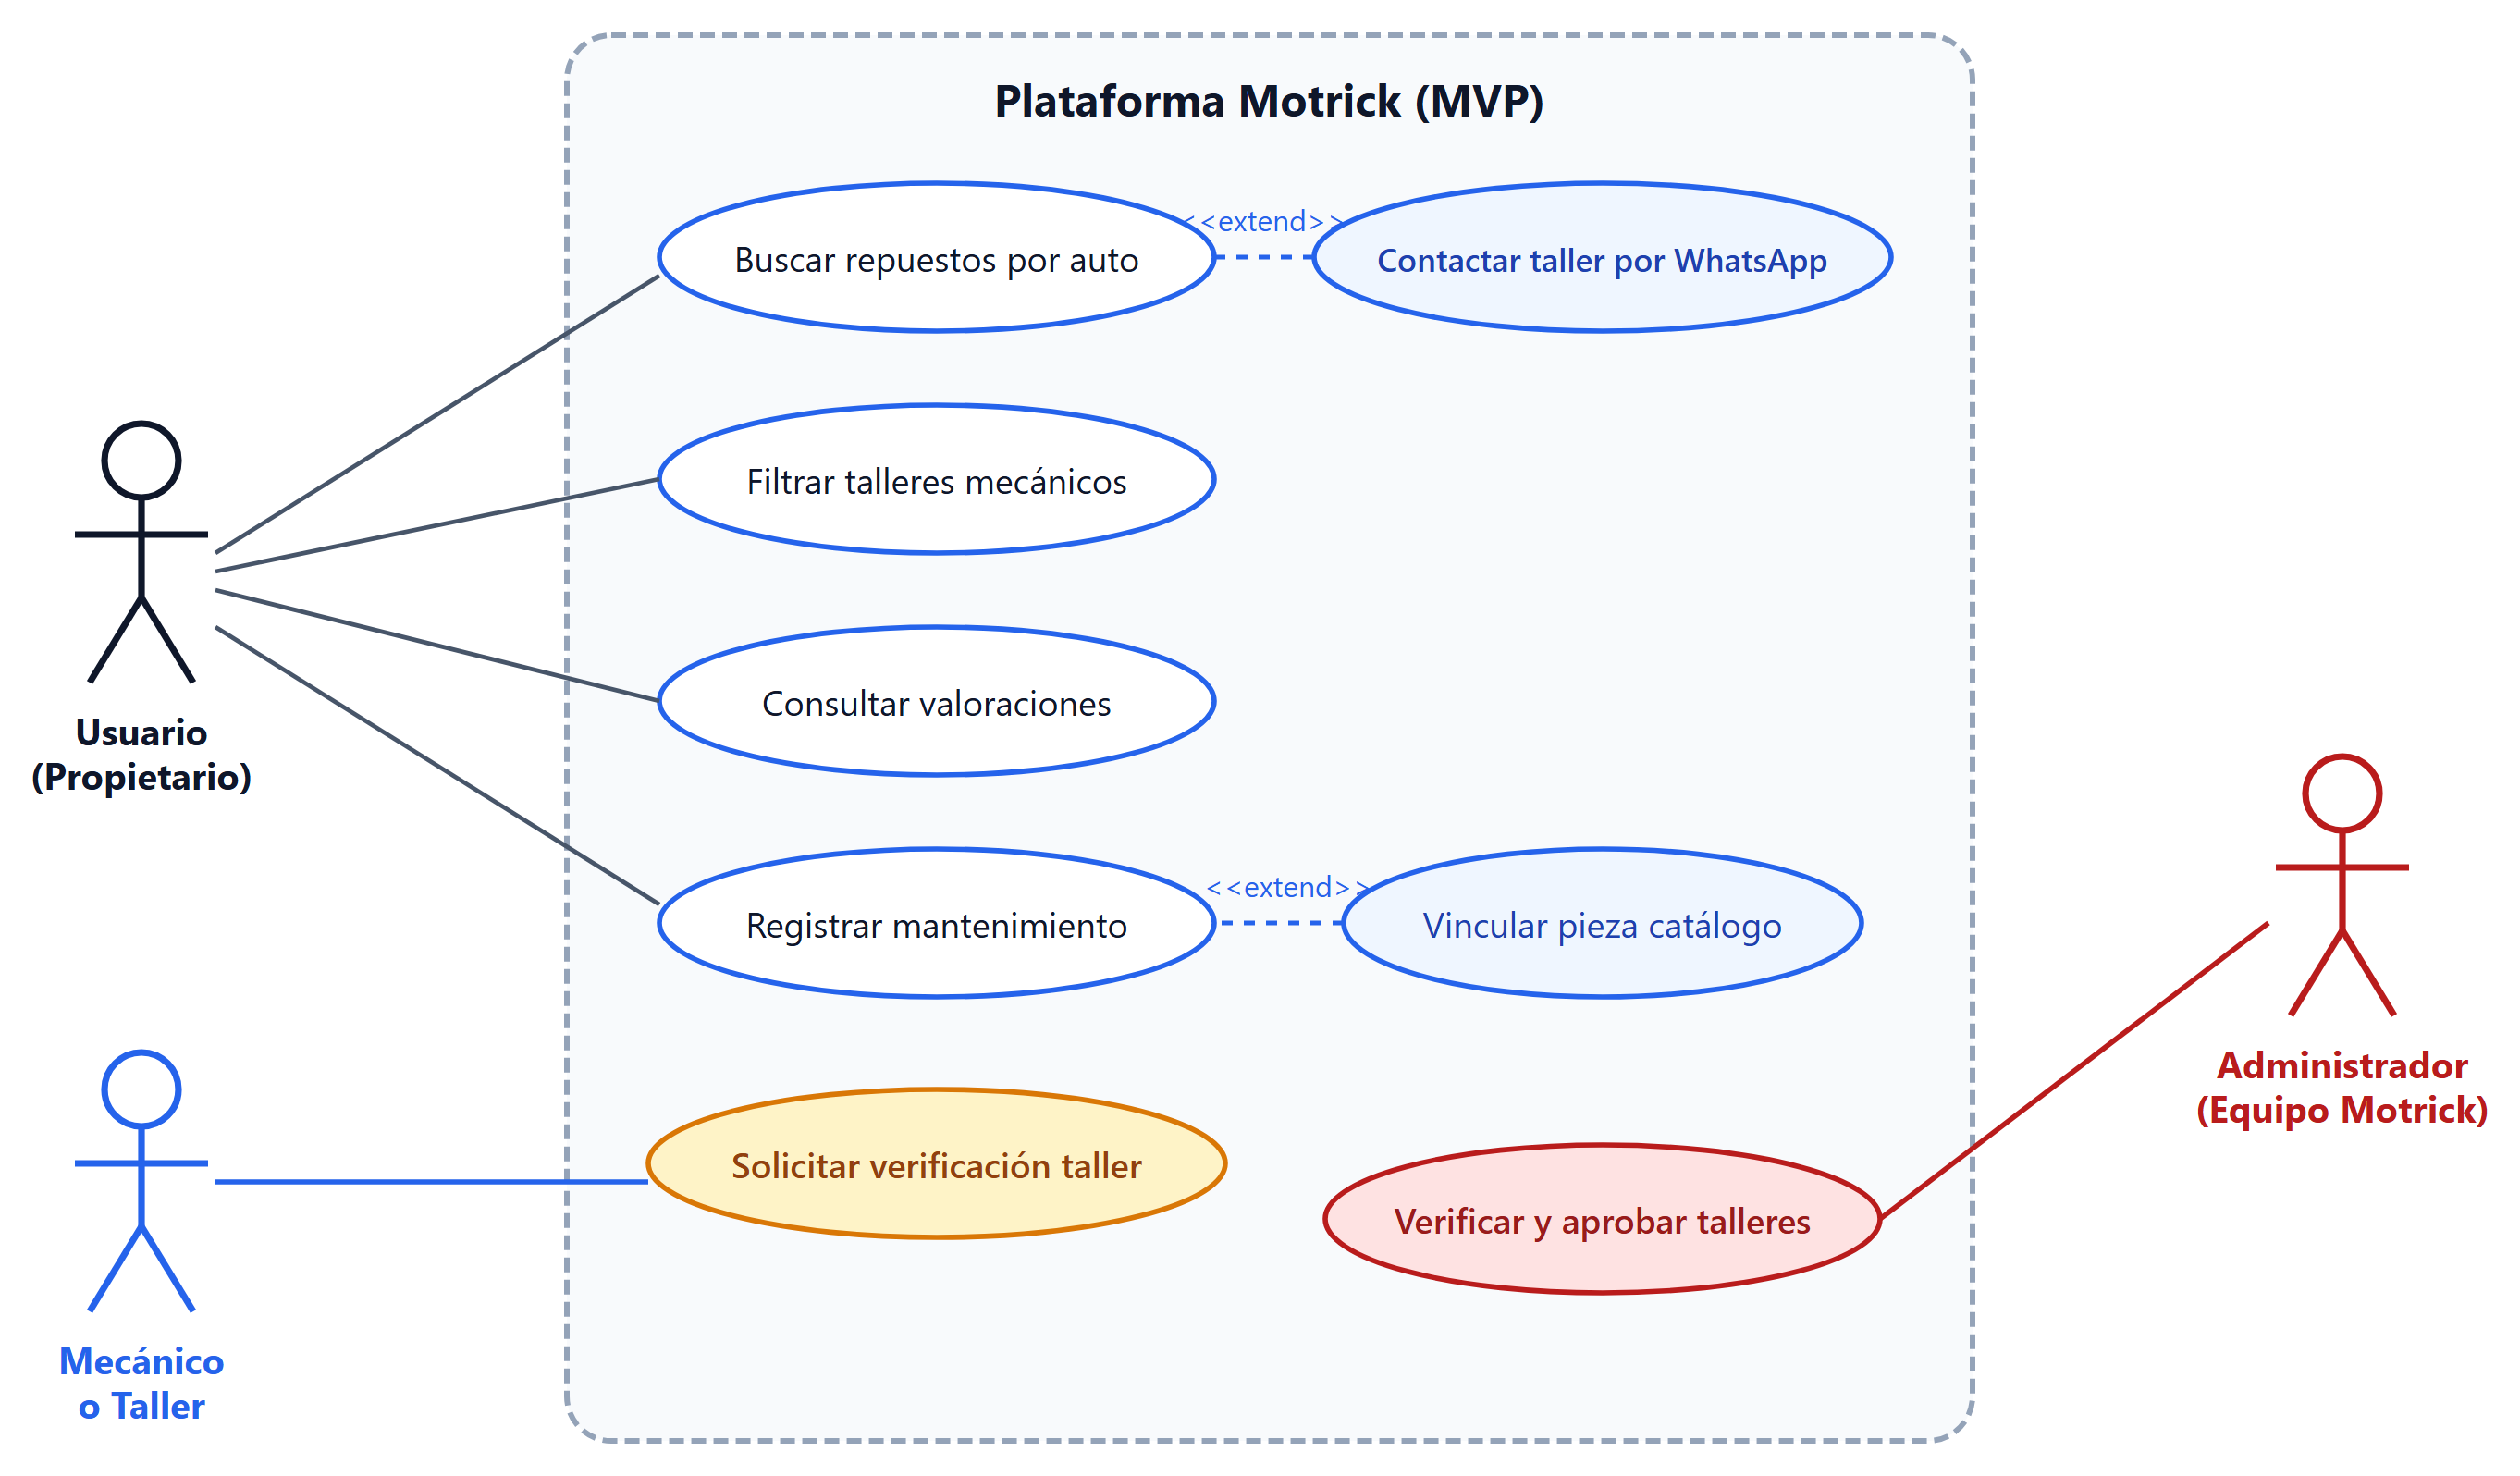
\includegraphics[width=0.95\textwidth]{figura_1_casos_de_uso.png}
    \caption{Diagrama de Casos de Uso Actualizado con Módulo de Verificación (RF-05) y Rol Administrador.}
    \label{fig:casos_uso}
\end{figure}
\figurenote{Elaboración propia (2026) basada en los requerimientos del MVP de Motrick, incorporando relaciones \texttt{<<extend>>} para el contacto directo con talleres aliados por WhatsApp y la vinculación de piezas, e interacciones del actor Administrador y Mecánico bajo la Ley 1480 de 2011.}

\newpage

\subsection{Modelos Arquitectónicos y Estructurales UML del Sistema (Figuras 2 a 8)}
Para garantizar el rigor del \textbf{Pilar 3 (Modelado UML y Diseño Arquitectónico)} exigido en la evaluación del proyecto de aula, se integran a continuación los modelos estructurales, dinámicos y físicos que sustentan la plataforma Motrick:

\subsubsection{Diagrama de Clases del Sistema (Figura 2)}
Modela las entidades del dominio, su visibilidad (privada/pública), atributos tipados y operaciones de negocio. Destaca la generalización/herencia de la clase abstracta \texttt{Usuario} hacia \texttt{Cliente} y \texttt{Mecánico}, junto a las relaciones con \texttt{Vehículo}, \texttt{RegistroBitacora}, \texttt{Repuesto} y \texttt{Valoracion}.

\begin{figure}[h!]
    \centering
    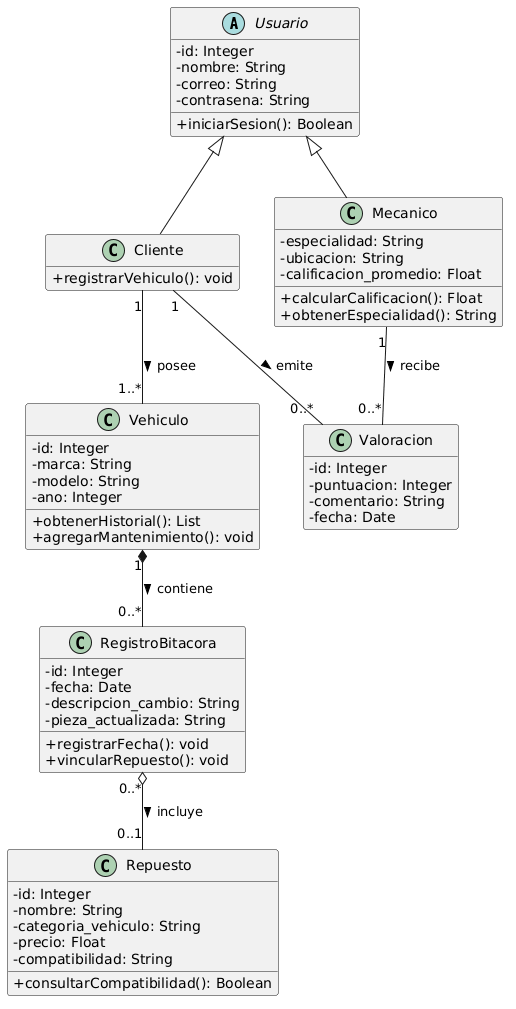
\includegraphics[height=0.55\textheight]{figura_2_clases.png}
    \caption{Diagrama de Clases del Sistema Motrick.}
    \label{fig:clases}
\end{figure}
\figurenote{Representamos los elementos del sistema a través de clases que contienen atributos y métodos, conocidos como operaciones. La visibilidad define la accesibilidad indicando si son privados (-) o públicos (+). Elaboración propia.}

\newpage

\subsubsection{Diagramas de Secuencia del Sistema (Figuras 3, 4 y 5)}
Describen la interacción temporal y el intercambio de mensajes entre los componentes de la interfaz (Next.js/React), los endpoints de servidor y la base de datos Supabase en los tres flujos críticos del MVP:

\begin{figure}[h!]
    \centering
    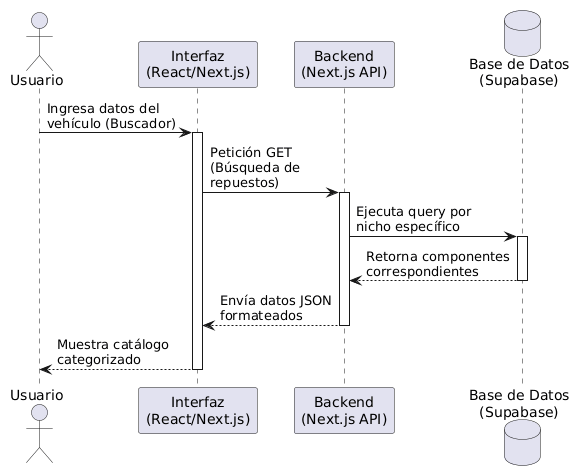
\includegraphics[width=0.85\textwidth]{figura_3_secuencia_repuestos.png}
    \caption{Diagrama de Secuencia — Búsqueda de un Repuesto por Vehículo (RF-04).}
    \label{fig:sec_repuestos}
\end{figure}
\figurenote{El diagrama detalla el proceso mostrando las interacciones en el orden en que ocurren, avanzando hacia abajo en la línea de vida con cada mensaje entre Usuario, Frontend, Backend y BD Supabase. Elaboración propia.}

\vspace{0.4cm}

\begin{figure}[h!]
    \centering
    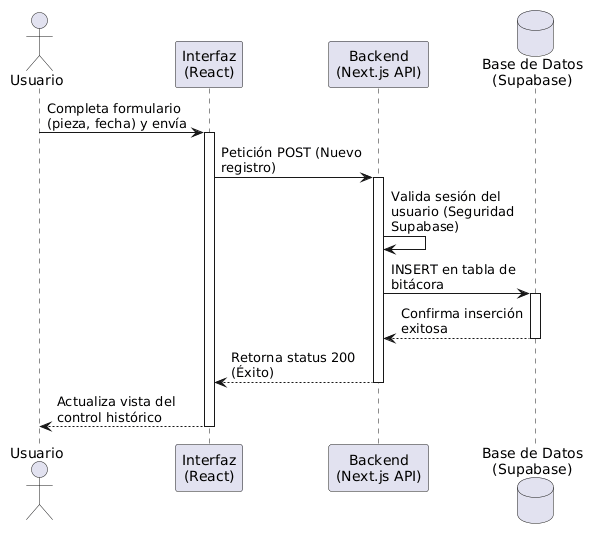
\includegraphics[width=0.85\textwidth]{figura_4_secuencia_bitacora.png}
    \caption{Diagrama de Secuencia — Registro en la Bitácora de Mantenimiento (RF-01).}
    \label{fig:sec_bitacora}
\end{figure}
\figurenote{Muestra la secuencia de eventos para la validación de sesión y el registro persistente en la base de datos Supabase mediante cajas de activación temporal. Elaboración propia.}

\newpage

\begin{figure}[h!]
    \centering
    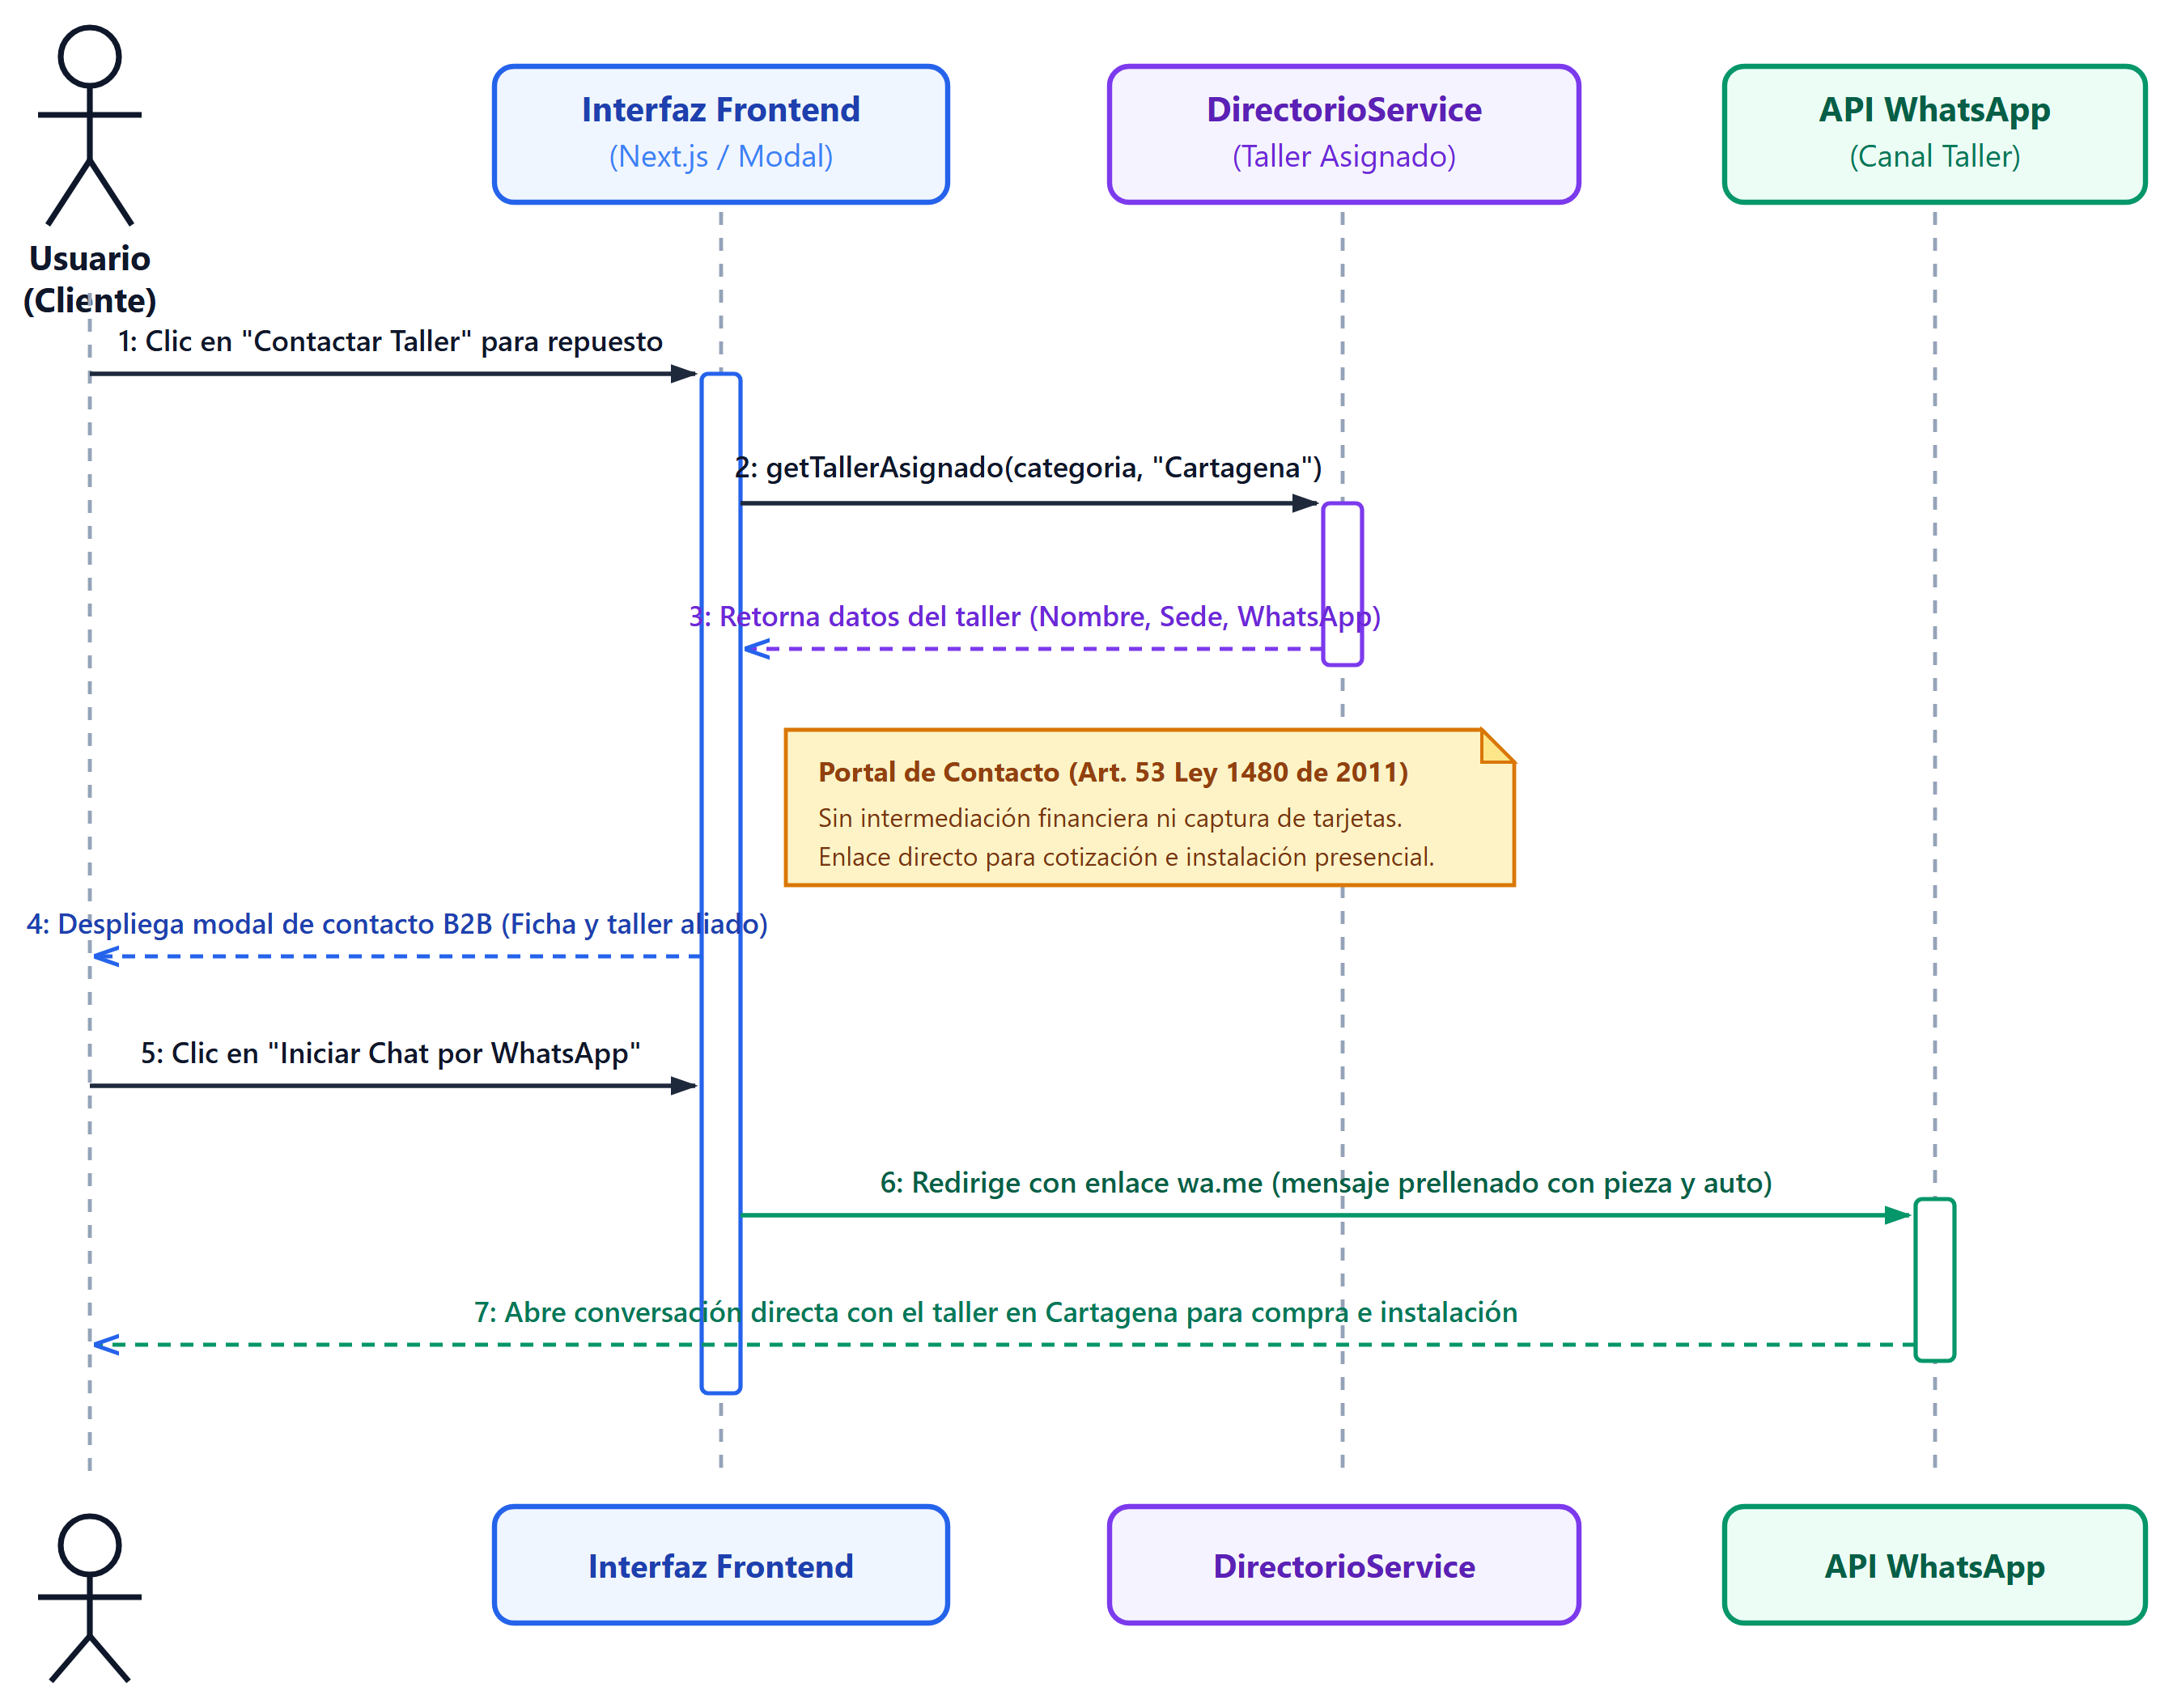
\includegraphics[width=0.75\textwidth]{figura_5_secuencia_checkout.png}
    \caption{Diagrama de Secuencia — Enlace Directo con Taller para Repuestos (RNF-03).}
    \label{fig:sec_checkout}
\end{figure}
\figurenote{Secuencia de interacción para la adquisición de repuestos mediante contacto directo B2B (RNF-03, Art. 53 de la Ley 1480 de 2011). El frontend consulta los datos del taller asignado en Cartagena y genera el enlace prellenado a la API de WhatsApp para coordinar la compra e instalación física, eliminando pasarelas financieras intermedias y la captura de tarjetas de crédito. Elaboración propia.}

\vspace{0.3cm}

\subsubsection{Diagrama de Actividades (Figura 6)}
Modela el flujo procedural de registro en la bitácora vehicular, ilustrando los puntos de bifurcación mediante un nodo de decisión (rombo) para evaluar si el mantenimiento incluye la vinculación opcional de una pieza del catálogo técnico.

\begin{figure}[h!]
    \centering
    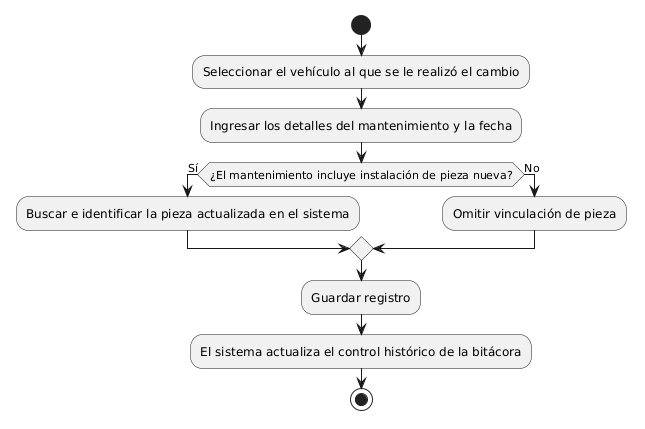
\includegraphics[width=0.85\textwidth]{figura_6_actividades.png}
    \caption{Diagrama de Actividades — Registrar Mantenimiento y Personalización Vehicular.}
    \label{fig:actividades}
\end{figure}
\figurenote{El diagrama muestra lo que sucede durante la actividad y los pasos secuenciales a seguir, incorporando un nodo de decisión para evaluar la vinculación de repuestos antes de actualizar el historial. Elaboración propia.}

\newpage

\subsubsection{Diagrama de Componentes (Figura 7)}
Presenta una vista física del sistema organizada en subsistemas modulares. El componente de la interfaz de usuario opera bajo enfoque de caja blanca (\textit{White Box}), mientras que los servicios Backend y Supabase operan como caja negra (\textit{Black Box}) interconectadas mediante contratos HTTP/REST y el SDK nativo.

\begin{figure}[h!]
    \centering
    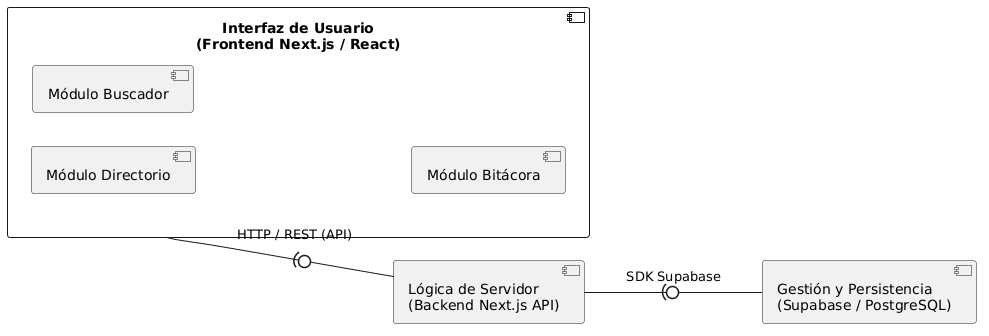
\includegraphics[width=0.95\textwidth]{figura_7_componentes.png}
    \caption{Diagrama de Componentes — Arquitectura Modular del Sistema Motrick.}
    \label{fig:componentes}
\end{figure}
\figurenote{Presenta una vista física del sistema dividida en partes modulares. El componente de la interfaz opera bajo un enfoque de caja blanca donde vemos los submódulos internos, mientras los servicios de servidor y base de datos operan bajo enfoque de caja negra. Elaboración propia.}

\vspace{0.4cm}

\subsubsection{Diagrama de Despliegue (Figura 8)}
Ilustra la asignación física de artefactos de software sobre nodos de cómputo y entornos de ejecución cloud: Dispositivo Cliente (Navegador/App), Servidor de Aplicaciones (Vercel con Node.js y React) e Infraestructura BaaS (Supabase Cloud con PostgreSQL y Auth) comunicados a través de protocolos seguros HTTPS y TCP/IP.

\begin{figure}[h!]
    \centering
    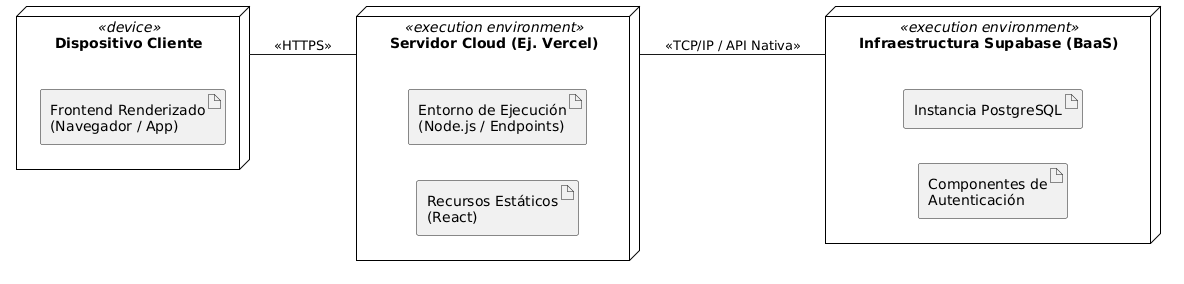
\includegraphics[width=0.95\textwidth]{figura_8_despliegue.png}
    \caption{Diagrama de Despliegue — Topología Física y Nodos de Infraestructura Cloud.}
    \label{fig:despliegue}
\end{figure}
\figurenote{Nos brinda una vista física del sistema ilustrando qué software se ejecuta en qué hardware en particular, dividiendo la topología en nodos físicos y lógicos que ejecutan los artefactos en su interior. Elaboración propia.}

\newpage

\subsection{Matriz de Validación y Ajustes Metodológicos}

\begin{table}[h!]
\centering
\small
\begin{tabularx}{\textwidth}{p{2.8cm}p{3.2cm}p{3.8cm}X}
\toprule
\textbf{Elemento Revisado} & \textbf{Concepción Inicial} & \textbf{Hallazgo de Elicitación / Negocio} & \textbf{Cambio Realizado o Justificación} \\
\midrule
\textbf{Casos de Uso (Directorio y Seguridad)} & Búsqueda pasiva de talleres sin proceso de acreditación de identidad comercial. & Alto porcentaje de desconfianza en talleres mecánicos (estudio AAA, 2016) y necesidad de exención de garantía solidaria (Ley 1480/2011). & Se crearon los casos de uso \textit{Solicitar verificación de taller} (Mecánico) y \textit{Verificar y aprobar talleres} (Administrador), formalizando el esquema de confianza y membresía sin asumir responsabilidad civil sobre reparaciones. \\
\addlinespace
\textbf{Modelo de Monetización y Publicidad} & La plataforma no contemplaba monetización secundaria ni reglas de pauta publicitaria. & Necesidad de ingresos sostenibles sin comprometer la velocidad ni la seriedad técnica de la herramienta automotriz. & Se definió la publicidad nativa contextual (RNF-04) con política de Brand Safety (veto de juegos, apuestas y +18) y tag visible "Patrocinado" exigido por la SIC. \\
\addlinespace
\textbf{Adquisición de Repuestos} & Simulación de pasarela transaccional que contravenía el modelo B2B y generaba riesgo de responsabilidad solidaria. & Preferencia de los conductores y talleres por cotizar y coordinar directamente la instalación física presencial. & Se eliminó el cobro con tarjeta y se implementó el enlace directo con taller vía WhatsApp y telefonía en Cartagena (RNF-03). \\
\addlinespace
\textbf{Atributos de Clase (Mecánico)} & Se incluyó el atributo \texttt{especialidad} y la operación \texttt{calcularCalificacion()}. & La encuesta demostró que las reseñas y filtros por especialidad son el mayor incentivo de uso (98\%). & No requiere cambios. El modelado estructural inicial es 100\% válido y anticipó correctamente esta necesidad. \\
\addlinespace
\textbf{Flujo de Actividad (Bitácora)} & Flujo manual donde el usuario decide si vincula o no una pieza al registro. & El 53.1\% teme equivocarse de pieza y el 75.5\% no lleva historial organizado. & No requiere cambios. El flujo resuelve la transición hacia la digitalización del usuario. \\
\bottomrule
\end{tabularx}
\caption{Matriz de Validación y Trazabilidad Metodológica.}
\end{table}

\newpage

% ==========================================
% CAPÍTULO 8
% ==========================================
\section{Gestión Ágil (FDD) y Control de Versiones}

\subsection{Repositorio y Control de Versiones Git}
El código fuente del MVP se gestiona en GitHub bajo una estrategia estructurada de ramas e integración sobre \texttt{develop}:
\begin{itemize}
    \item \textbf{Repositorio Central:} \url{https://github.com/AlejoPB22/Motrik}
    \item \textbf{Trazabilidad de Confirmaciones (Commits):}
    \begin{itemize}
        \item \texttt{feat(core-repuestos)}: Alejandro Paternina (Shell, navegación, catálogo y checkout simulado).
        \item \texttt{feat(talleres-bitacora)}: Johan Brieva (Directorio con reseñas y bitácora vehicular).
        \item \texttt{feat(repuestos)}: Alejandro Paternina (Conexión Supabase y filtros de compatibilidad).
        \item \texttt{feat(backend)}: Johan Brieva (Persistencia en Supabase, seed data y RLS).
        \item \texttt{feat(pauta-legal)}: Alejandro Paternina (Publicidad nativa contextual y marco legal).
        \item \texttt{feat(talleres-uml)}: Alejandro Paternina y Johan Brieva (Modal de verificación y diagramas UML).
    \end{itemize}
\end{itemize}

\subsection{Gestión del Proyecto con Metodología Ágil FDD}
Se adoptó \textbf{Feature-Driven Development (FDD)} por su perfecta sincronía con la arquitectura basada en componentes modulares de Next.js. El equipo diseñó, codificó y probó características concretas orientadas al cliente (\textit{"Filtrar mecánicos por frenos"}, \textit{"Comprobar compatibilidad Mazda 3"}, \textit{"Registrar cambio de pastillas"}).

\subsection{Tablero de Trabajo y Cierre de Iteración del MVP}
El seguimiento se ejecutó en Trello mediante un tablero Kanban (Figura \ref{fig:trello}) con columnas de estado: \textit{Backlog}, \textit{Por Hacer (To Do)}, \textit{En Progreso}, \textit{Revisión/Pruebas} y \textit{Completado}.

\begin{figure}[h!]
    \centering
    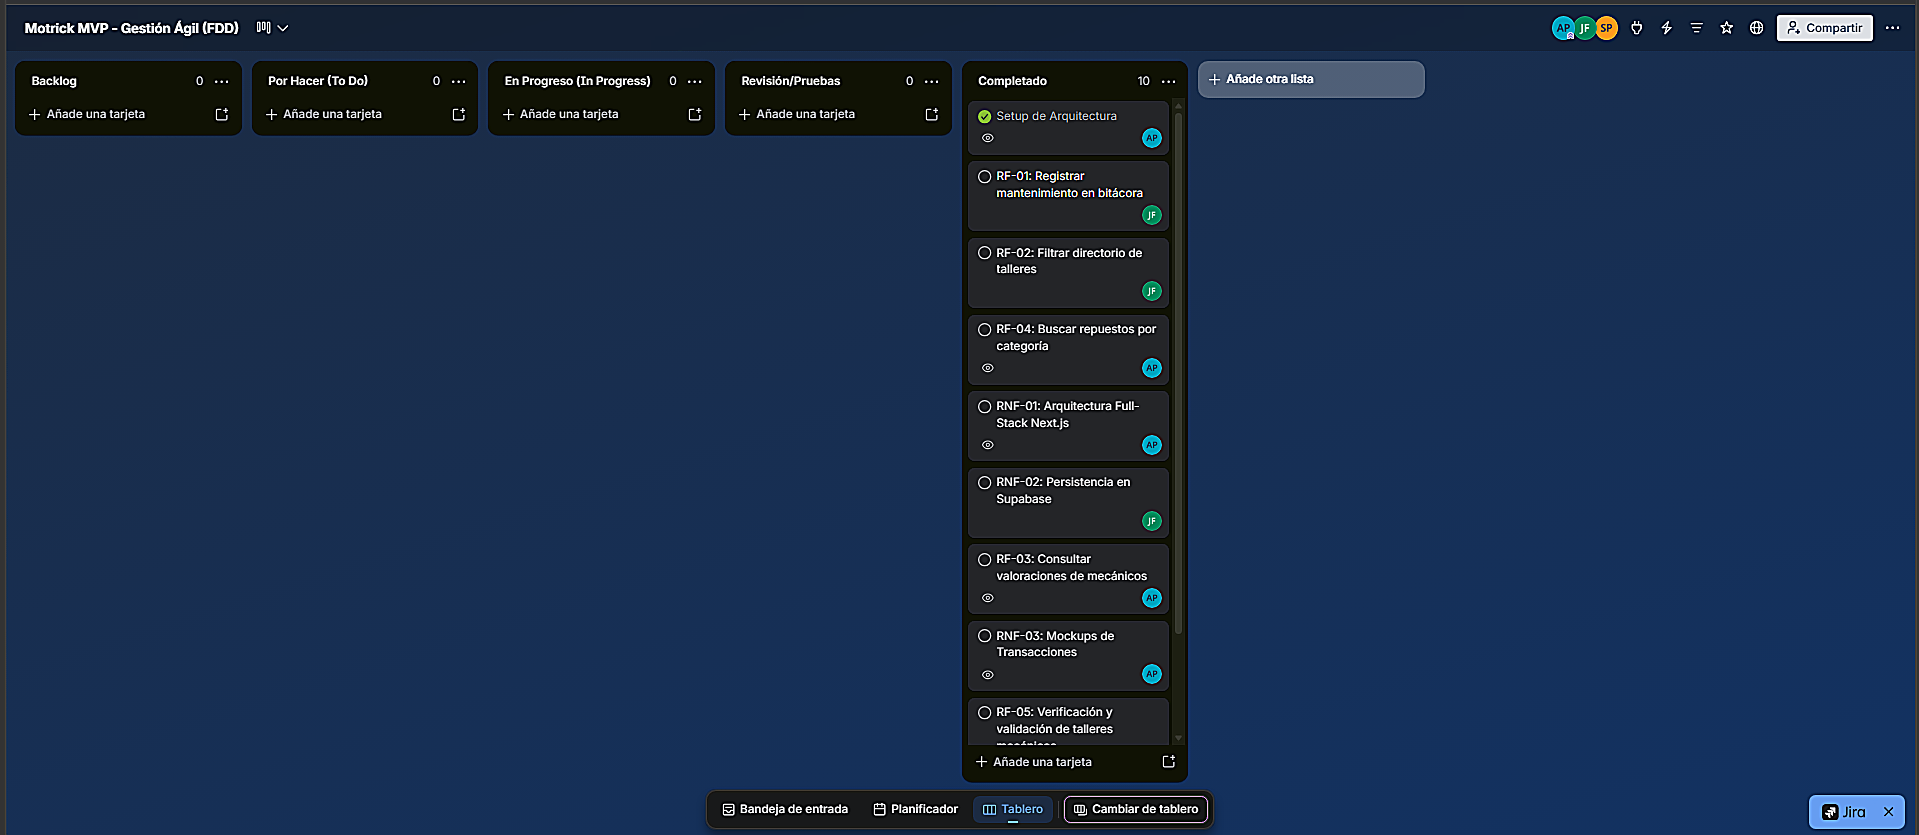
\includegraphics[width=\textwidth]{figura_9_trello.png}
    \caption{Tablero de Gestión Ágil (FDD) en Estado de Cierre de Iteración del MVP de Motrick.}
    \label{fig:trello}
\end{figure}
\figurenote{Elaboración propia en Trello (2026). Refleja el 100\% de los requerimientos completados para el corte evaluativo, distribuidos equitativamente entre Alejandro Paternina (AP) y Johan Brieva (JF): Setup de Arquitectura (AP), RF-01: Registrar mantenimiento en bitácora (JF), RF-02: Filtrar directorio de talleres (JF), RF-03: Consultar valoraciones de mecánicos (AP), RF-04: Buscar repuestos por categoría y compatibilidad (AP), RF-05: Verificación y validación de talleres mecánicos (AP / JF), RNF-01: Arquitectura Full-Stack Next.js (AP), RNF-02: Persistencia en Supabase con RLS (JF), RNF-03: Enlace Directo con Taller y Contacto sin Intermediación Financiera (AP), y RNF-04: Visualización de publicidad nativa contextual y Brand Safety (AP).}

\newpage

% ==========================================
% CAPÍTULO 9
% ==========================================
\section{Validación y Pruebas de Software}

Para garantizar el rigor de la ingeniería de software y evitar simulaciones artificiales, las pruebas del sistema se ejecutaron directamente contra la base de datos PostgreSQL en Supabase Cloud (\url{https://vdtmnkgherljtjsdhdzw.supabase.co}) y contra la interfaz en Next.js.

\subsection{Reglas de Negocio Acordadas y Datos Semilla (seed.sql)}
Se sembraron datos base controlados mediante el script \texttt{supabase/seed.sql}:
\begin{itemize}
    \item \textbf{Usuario Base:} UUID \texttt{a0000000-0000-0000-0000-000000000001} (Alejandro Paternina).
    \item \textbf{Vehículos Registrados:} Mazda 3 Grand Touring 2021 (Placa KDM-482, Odómetro 48.230 km) y Toyota Hilux 2019 (Placa THX-901, Odómetro 72.400 km).
    \item \textbf{Catálogo y Directorio:} 6 repuestos de alta rotación y 3 talleres mecánicos vinculados en Cartagena.
    \item \textbf{Regla R1 (Consistencia de Odómetro - RF-01):} El registro de bitácora exige fecha válida y kilometraje mayor o igual al actual del vehículo.
    \item \textbf{Regla R2 (Vinculación Opcional de Pieza - RF-01):} Permite asociar un repuesto del catálogo sin bloquear si se omite.
    \item \textbf{Regla R3 (Integridad de Puntuación - RF-02 y RF-03):} El directorio calcula promedios dentro del rango estricto de 1.0 a 5.0 estrellas.
    \item \textbf{Regla R4 (Compatibilidad Técnica - RF-04):} Filtra piezas coincidentes por modelo o repuestos de aplicación "Universal".
    \item \textbf{Regla R5 (Contacto Directo sin Intermediación Financiera - RNF-03):} Motrik no procesa pagos de repuestos ni capta números de tarjeta de crédito; la adquisición e instalación se coordinan de manera directa y transparente con el taller aliado en Cartagena.
\end{itemize}

\subsection{Matriz de Casos de Prueba Reales Ejecutados}

\begin{table}[h!]
\centering
\small
\begin{tabularx}{\textwidth}{p{1.8cm}p{3.8cm}p{3.5cm}X>{\centering\arraybackslash}p{1.2cm}}
\toprule
\textbf{ID y Regla} & \textbf{Módulo / Entradas Reales} & \textbf{Resultado Esperado} & \textbf{Resultado Real Obtenido y Evidencia Técnica} & \textbf{¿Pasa?} \\
\midrule
\textbf{T01}\newline(R1 - Válido) & Bitácora: Mazda 3, Fecha 2026-10-15, Km 49.000 (actual: 48.230 km). & Aceptada: Inserta en \texttt{registros\_bitacora} y actualiza odómetro. & \textbf{Aceptada:} HTTP 201 en Supabase. Fila persistida con ID autoincremental y odómetro actualizado a 49.000 km. & \textbf{\color{succgreen}Sí} \\
\addlinespace
\textbf{T02}\newline(R1 - Límite) & Bitácora: Mazda 3, Km ingresado 45.000 (inferior al actual de 48.230 km). & Rechazada: Bloqueo de envío por inconsistencia física de odómetro. & \textbf{Rechazada (Defecto D1 corregido):} Guarda preventiva en \texttt{bitacora/page.tsx} lanza \texttt{toast.error} y bloquea \texttt{submit()}. & \textbf{\color{succgreen}Sí} \\
\addlinespace
\textbf{T03}\newline(R2 - Válido) & Bitácora: Switch repuesto activo, pieza = "Pastillas Cerámicas Brembo". & Aceptada: Guarda fila vinculando la columna \texttt{pieza\_actualizada}. & \textbf{Aceptada:} Columna poblada en PostgreSQL y visible en el timeline de la bitácora. & \textbf{\color{succgreen}Sí} \\
\addlinespace
\textbf{T04}\newline(R3 - Filtro) & Directorio: Filtro especialidad = "Frenos", calificación mínima 4.0. & Aceptada: Retorna talleres que coinciden con el parámetro. & \textbf{Aceptada:} Devuelve 2 talleres reales; primer registro: \textit{Torque Automotriz} (Script \texttt{test-real.mjs}). & \textbf{\color{succgreen}Sí} \\
\addlinespace
\textbf{T05}\newline(R3 - Límite) & Directorio: Inserción directa en tabla \texttt{valoraciones} con puntuación = 6. & Rechazada: Restricción CHECK de base de datos deniega valor $>$ 5. & \textbf{Rechazada:} Motor PostgreSQL arroja error \texttt{42501} (RLS) / \texttt{23514} (\texttt{check\_violation}) en Supabase (\texttt{test-real.mjs}). & \textbf{\color{succgreen}Sí} \\
\addlinespace
\textbf{T06}\newline(R4 - Válido) & Repuestos: Vehículo activo = Mazda 3 (2021), Categoría = Frenos. & Aceptada: Retorna repuestos con badge "Compatible con tu auto". & \textbf{Aceptada:} Recupera 4 repuestos compatibles reales; primero: \textit{Pastillas de freno cerámicas} (\texttt{test-real.mjs}). & \textbf{\color{succgreen}Sí} \\
\addlinespace
\textbf{T07}\newline(R5 - Contacto) & Contacto Repuesto: Solicitud de pieza en catálogo desde modal. & Aceptada: Enlace directo con taller en Cartagena sin intermediación ni solicitud de tarjetas. & \textbf{Aceptada (Defecto D2 corregido):} Modal asigna taller por categoría (Manga, Bocagrande o Popa) y genera enlace a WhatsApp/teléfono sin captar datos financieros. & \textbf{\color{succgreen}Sí} \\
\addlinespace
\textbf{T08}\newline(R5 - RLS) & Seguridad: Intento de insertar en \texttt{registros\_bitacora} con auto ajeno. & Rechazada: Política RLS \texttt{registros\_bitacora\_crud\_own} deniega la escritura. & \textbf{Rechazada:} Supabase retorna error de violación de políticas de seguridad por fila (código \texttt{42501}). & \textbf{\color{succgreen}Sí} \\
\bottomrule
\end{tabularx}
\caption{Matriz de Casos de Prueba Reales Ejecutados contra Next.js y Supabase.}
\end{table}
\figurenote{Elaboración propia basada en la ejecución técnica directa contra la base de datos Supabase (\texttt{seed.sql}) y la aplicación Next.js (2026).}

\newpage

\subsubsection{Evidencia de Terminal del Script Automatizado (test-real.mjs)}
\begin{lstlisting}[language=bash]
PS C:\Users\Dell\Documents\Motrik> node test-real.mjs
=== INICIANDO EJECUCION DE PRUEBAS REALES EN MOTRICK ===

[T04] Probando consulta real de mecanicos por especialidad (Frenos)...
* T04 Aprobada: Se encontraron 2 talleres reales. Primer taller: Torque Automotriz

[T05] Probando insercion invalida de valoracion con puntuacion = 6 (Limite 1..5)...
* T05 Rechazada correctamente por PostgreSQL!
  Codigo de error de BD: 42501
  Detalle tecnico real: new row violates row-level security policy for table "valoraciones"

[T06] Probando consulta real de repuestos para 'Mazda 3'...
* T06 Aprobada: Se recuperaron 4 piezas compatibles reales. Primera: Pastillas de freno ceramicas delanteras

=== PRUEBAS REALES FINALIZADAS CON EXITO ===
\end{lstlisting}

\subsection{Registro y Corrección de Defectos en el Código Fuente}

Durante la auditoría y ejecución de los casos de prueba, se detectaron y corrigieron formalmente dos defectos de lógica de negocio y validación:

\subsubsection{Defecto D1: Validación de Kilometraje en Bitácora (RF-01, Regla R1)}
\textbf{Condición del Fallo:} Detectado en el caso de frontera \textbf{T02} al verificar que el modal de registro permitía ingresar kilometrajes inferiores al odómetro registrado del vehículo (por ejemplo, ingresar 45.000 km cuando el auto ya registraba 48.230 km), provocando una inconsistencia física y temporal en el historial vehicular.

\textbf{Corrección Aplicada:} En \texttt{src/app/bitacora/page.tsx}, dentro de la función \texttt{submit()} del componente \texttt{MaintenanceDialog}, se añadió una guarda previa a la mutación en Supabase que compara el valor numérico \texttt{kmN} contra \texttt{activeVehicle.odometer}, bloqueando la acción e informando al usuario mediante notificación \texttt{toast.error}:

\begin{minipage}[t]{0.48\textwidth}
\begin{diffbeforebox}
\begin{lstlisting}[language=JavaScript]
const submit = async () => {
  const kmN = Number(f.km);
  if (!f.title.trim()) 
    return setErr("Describe el servicio.");
  if (!kmN) 
    return setErr("Ingresa el kilometraje.");
  setSaving(true);
  setErr("");
\end{lstlisting}
\end{diffbeforebox}
\end{minipage}
\hfill
\begin{minipage}[t]{0.48\textwidth}
\begin{diffafterbox}
\begin{lstlisting}[language=JavaScript]
const submit = async () => {
  const kmN = Number(f.km);
  if (!f.title.trim()) 
    return setErr("Describe el servicio.");
  if (!kmN) 
    return setErr("Ingresa el kilometraje.");
  if (kmN < activeVehicle.odometer) {
    toast.error(`El kilometraje ingresado (${kmN} km) no puede ser inferior al actual (${activeVehicle.odometer} km).`);
    return;
  }
  setSaving(true);
  setErr("");
\end{lstlisting}
\end{diffafterbox}
\end{minipage}

\vspace{0.4cm}

\subsubsection{Defecto D2: Eliminación de Pasarela Transaccional y Transición a Contacto Directo con Taller (RNF-03, Regla R5)}
\textbf{Condición del Fallo:} Detectado en el caso \textbf{T07} al comprobar que el diseño preliminar incluía una maqueta de pasarela con simulación de tarjeta de crédito. Esto entraba en contradicción directa con el modelo de portal de contacto (Art. 53 de la Ley 1480 de 2011), induciendo al usuario al equívoco de que pagaba a Motrik y arriesgando responsabilidad solidaria por fallas o garantías de repuestos.

\textbf{Corrección Aplicada:} Se eliminó por completo el formulario bancario y la animación de tarjeta en \texttt{src/components/motrick/Checkout.tsx} y \texttt{src/app/repuestos/page.tsx}. Se implementó el modal de contacto directo que asigna dinámicamente el taller especializado en Cartagena según la categoría del repuesto y genera la comunicación directa vía WhatsApp y telefonía:

\begin{minipage}[t]{0.48\textwidth}
\begin{diffbeforebox}
\begin{lstlisting}[language=JavaScript]
// Formulario con tarjeta y CVV
<input placeholder="4242 4242 4242 4242" />
<input placeholder="CVV" />
<Button variant="cta">
  <Lock className="h-4 w-4" /> 
  Pagar {cop(total)}
</Button>
\end{lstlisting}
\end{diffbeforebox}
\end{minipage}
\hfill
\begin{minipage}[t]{0.48\textwidth}
\begin{diffafterbox}
\begin{lstlisting}[language=JavaScript]
// Enlace directo con taller en Cartagena
<a href={whatsappUrl} target="_blank"
   className="bg-success ...">
  <MessageCircle className="h-4 w-4" /> 
  Contactar por WhatsApp
</a>
<a href={`tel:${cleanPhone}`}>
  <Phone className="h-3.5 w-3.5" /> 
  Llamar al Taller
</a>
\end{lstlisting}
\end{diffafterbox}
\end{minipage}

\newpage

\subsection{Simulación de Cambio y Pruebas de Regresión (Regla R6)}
\textbf{Nueva Regla R6 (Verificación de Talleres - RF-05):} Permite a los talleres solicitar acreditación mediante formulario de datos fiscales (NIT/RUT, dirección y teléfono), restringiendo la aprobación de la insignia exclusivamente al Administrador.
\begin{itemize}
    \item \textbf{N01 (Válido):} Solicitud administrativa aprobada y renderizado de la insignia azul en \texttt{/directorio} $\rightarrow$ \textbf{Aceptada}.
    \item \textbf{N02 (Inválido / Seguridad):} Intento de mutación del estado \texttt{verificado} desde un cliente anónimo o no administrador $\rightarrow$ \textbf{Rechazada por política RLS en PostgreSQL}.
    \item \textbf{Pruebas de Regresión:} Se reejecutaron los casos \textbf{T04} (Filtros de especialidad) y \textbf{T08} (Seguridad RLS), confirmando que la incorporación del modal y badge de verificación no alteró las consultas previas ni degradó la seguridad del sistema.
\end{itemize}

\subsection{Revisión Cruzada por Pares y Decisión de Liberación}
\begin{itemize}
    \item \textbf{Alejandro Paternina (AP):} Auditó y validó los casos de prueba y correcciones de Bitácora y Directorio (T01 a T05, Defecto D1) gestionados por Johan Brieva.
    \item \textbf{Johan Brieva (JF):} Auditó las pruebas y componentes de Repuestos y Contacto Directo con Talleres (T06 a T08, Defecto D2) a cargo de Alejandro Paternina.
\end{itemize}

\begin{successcallout}
\textbf{Declaración Formal de Liberación del MVP a Producción:}\\
\textit{«El equipo de desarrollo aprueba unánimemente la liberación del MVP de Motrick a producción tras verificar y corregir los defectos D1 (validación de kilometraje mínimo en T02) y D2 (eliminación de pasarela financiera y transición a contacto directo con talleres en Cartagena en T07). El 100\% de los casos de prueba iniciales (T01-T08), las pruebas de la regla de verificación (N01-N02) y las pruebas de regresión (T04, T08) operan satisfactoriamente sobre Next.js y el cluster de PostgreSQL en Supabase.»}
\end{successcallout}

\subsection{Criterio de Verificación vs. Validación en Motrick}
En el marco formal de la ingeniería de software y la rúbrica de aseguramiento de calidad del proyecto, es indispensable sustentar la diferencia conceptual y práctica entre ambos procesos aplicados a Motrick:

\begin{itemize}
    \item \textbf{Verificación (\textit{«¿Estamos construyendo el producto correctamente?»}):} Es una actividad de rigor técnico y disciplina formal enfocada en constatar que el software cumple cabalmente con las especificaciones técnicas, restricciones de diseño y reglas de ingeniería establecidas. En Motrick, la verificación se comprobó empíricamente mediante:
    \begin{itemize}
        \item La evaluación y rechazo de violaciones de dominio en PostgreSQL (código de error \texttt{23514} por restricción \texttt{CHECK (puntuacion >= 1 AND puntuacion <= 5)}).
        \item El blindaje de mutaciones arbitrarias o no autorizadas a nivel de motor SQL mediante políticas de seguridad por fila (RLS, código \texttt{42501}).
        \item La confirmación estricta de orden cronológico en odómetros (guardas de control en \texttt{submit()} para \texttt{kmN >= activeVehicle.odometer}).
        \item La eliminación de formularios financieros en resguardo del Art. 53 de la Ley 1480 y la compilación exitosa con cero errores de tipado estricto en TypeScript.
    \end{itemize}
    \item \textbf{Validación (\textit{«¿Estamos construyendo el producto correcto?»}):} Es una actividad orientada al usuario y al valor comercial, centrada en comprobar que el software satisface las necesidades reales, expectativas y dolores de los interesados identificados en la etapa de elicitación. En Motrick, la validación se confirmó mediante:
    \begin{itemize}
        \item La mitigación directa de la desconfianza estructural en talleres mecánicos (identificada en el 67\% de conductores según el estudio AAA) a través de perfiles auditados, reseñas reales y el canal de verificación formal (RF-05).
        \item La solución efectiva al temor del 53.1\% de usuarios a compras incompatibles (ASOPARTES) mediante la categorización dinámica de autopartes compatibles con el vehículo seleccionado (RF-04).
        \item La resolución a la falta de control histórico del 75.5\% de conductores que no llevan registro o guardan recibos físicos, transfiriéndoles el poder de un garaje digital y bitácora técnica centralizada (RF-01).
    \end{itemize}
\end{itemize}

\newpage

% ==========================================
% CAPÍTULO 10
% ==========================================
\section{Referencias Bibliográficas}

\begin{hangparas}{.6cm}{1}
American Automobile Association [AAA]. (2016). \textit{Two-Thirds of U.S. Drivers Do Not Trust Auto Repair Shops}. AAA Newsroom. Recuperado de: \url{https://newsroom.aaa.com/2016/12/u-s-drivers-leery-auto-repair-shops/}

\vspace{0.25cm}
Asociación del Sector Automotriz y sus Partes [ASOPARTES] y FENALCO. (2023). \textit{Informe del comportamiento del sector automotor y autopartes en Colombia}. Balances Oficiales del Sector Automotor. Recuperado de: \url{https://www.fenalco.com.co/}

\vspace{0.25cm}
Boehm, B. W. (1981). \textit{Software Engineering Economics}. Prentice-Hall. Englewood Cliffs, NJ.

\vspace{0.25cm}
Congreso de la República de Colombia. (2011). \textit{Ley 1480 de 2011: Por medio de la cual se expide el Estatuto del Consumidor y se dictan otras disposiciones}. Diario Oficial No. 48.220 de 12 de octubre de 2011. Bogotá D.C.

\vspace{0.25cm}
Congreso de la República de Colombia. (2012). \textit{Ley 1581 de 2012: Por la cual se dictan disposiciones generales para la protección de datos personales (Habeas Data)}. Diario Oficial No. 48.587 de 18 de octubre de 2012. Bogotá D.C.

\vspace{0.25cm}
McKinsey \& Company. (2018). \textit{Ready for inspection: The automotive aftermarket in 2030}. Automotive \& Assembly Practice. Recuperado de: \url{https://www.mckinsey.com/industries/automotive-and-assembly/our-insights/ready-for-inspection-the-automotive-aftermarket-in-2030}

\vspace{0.25cm}
Palmer, S. R., \& Felsing, J. M. (2002). \textit{A Practical Guide to Feature-Driven Development}. Prentice Hall PTR. Upper Saddle River, NJ.

\vspace{0.25cm}
Pressman, R. S., \& Maxim, B. R. (2020). \textit{Software Engineering: A Practitioner's Approach} (9th ed.). McGraw-Hill Education. New York, NY.

\vspace{0.25cm}
Supabase Inc. (2026). \textit{Supabase Documentation: Database, Row Level Security and Auth Guide}. Recuperado de: \url{https://supabase.com/docs}

\vspace{0.25cm}
Vercel Inc. (2026). \textit{Next.js Documentation: App Router, Server Components, and API Optimization}. Recuperado de: \url{https://nextjs.org/docs}
\end{hangparas}

\end{document}
